%\documentclass{iesbs}
\documentclass{amsart}
\usepackage{latexsym}
\usepackage{lscape}
\usepackage{graphics}
\usepackage{alltt}
\setcounter{secnumdepth}{3}
\setcounter{tocdepth}{3}
\setlength{\textwidth}{135mm}
\setlength{\textheight}{200mm}
\setlength{\oddsidemargin}{10mm}
\setlength{\evensidemargin}{10mm}
\setlength{\topmargin}{0mm}
\setlength{\textwidth}{6in}
\renewcommand{\abstractname}{Abstract}
\newtheorem{assumption}{Assumption}
\newtheorem{lemma}{Lemma}[section]
\newtheorem{theorem}{Theorem}[section]
\def\sT{\scriptscriptstyle T}
\def\RR{\hbox{\raise.4ex\hbox{$\scriptstyle{|}$}\hskip-1.85pt R}}
\def\OO{\mathcal O}
\def\SS{\mathcal S}
\def\argmin{\mathrm{argmin}}
\newcommand{\Jureckova}{Jure\v{c}kov\'{a} }
\newcommand{\Hajek}{H\'{a}jek }
\newcommand{\Hardle}{H\"{a}rdle }
\newcommand{\Sidak}{\v{S}id\'{a}k }


\newenvironment{apabib}{
  \noindent
\begin{center}
{\bf{ R}EFERENCES}
\end{center}
\vspace{-3mm}
\begin{list}{}{
  \topsep          0mm
  \leftmargin     10mm
  \parsep          0mm
  \listparindent -10mm}
  \item[]\strut\par}{
\end{list}}
 

\begin{document}
\title{Quantile Regression }
\thanks{
Version: {\today}.
This article has been prepared for the statistics section of the
{\it International Encyclopedia of the Social Sciences}
edited by Stephen Fienberg and Jay Kadane.
The research was partially supported by NSF grant SBR-9617206.
}



\author{Roger Koenker}

\begin{abstract}
Classical least squares regression may be viewed as a
natural way of extending the idea of estimating an unconditional
mean parameter to the problem of estimating conditional mean {\it functions};
the crucial link is the formulation of an optimization problem
that encompasses both problems.  Likewise, quantile regression
offers an extension of univariate quantile estimation to estimation
of conditional quantile functions via an optimization of
a piecewise linear objective function in the residuals.  Median
regression minimizes the sum of absolute residuals, an idea introduced
by Boscovich in the 18th century.

The asymptotic theory of quantile regression closely parallels the
theory of the univariate sample quantiles. Computation
of quantile regression estimators may be formulated as a linear
programming problem and efficiently solved by simplex or
barrier methods.  A close link to rank based inference has been
forged from the theory of the dual regression quantile process,
or regression rankscore process.
\end{abstract}

\maketitle

Quantile regression is a statistical technique intended to estimate,
and conduct inference about, conditional quantile functions. 
Just as classical linear regression methods based on
minimizing sums of squared residuals enable one to estimate models for
conditional mean functions, quantile regression methods offer a mechanism
for estimating models for the conditional median function, and the full
range of other conditional quantile functions.
By supplementing the estimation of conditional mean functions with
techniques for estimating an entire family of conditional quantile
functions, quantile regression is capable of providing a more
complete statistical analysis of the stochastic relationships among
random variables.

Quantile regression has been used in a broad range of application settings.
Reference growth curves for childrens' height and weight have a long history
in pediatric medicine; quantile regression methods may be used to estimate
upper and lower quantile reference curves as a function of age, sex, and
other covariates without imposing stringent parametric assumptions on the
relationships among these curves.  Quantile regression methods have been
widely used in economics to study determinents of wages, discrimination
effects, and trends in income inequality.  
Several recent studies have modeled the performance of public school
students on standardized exams as a function of socio-economic characteristics
like their parents' income and educational attainment, and policy variables 
like class size, school expenditures, and teacher qualifications.  It seems
rather implausible that such covariate effects should all act so as to
shift the entire distribution of test results by a fixed amount.
It is of obvious interest to know whether policy interventions alter
performance of the strongest students in the same way that weaker students
are affected.  Such questions are naturally investigated within the quantile
regression framework.  

In ecology, theory often suggests
how observable covariates affect limiting sustainable population sizes, and
quantile regression has been used to directly estimate models for upper 
quantiles of the conditional distribution rather than inferring such
relationships from models based on conditional central tendency.  In
survival analysis, and event history analysis more generally, there is
often also a desire to focus attention on particular segments of the
conditional distribution, for example survival prospects of the oldest-old,
without the imposition of global distributional assumptions.  



\section{Quantiles, Ranks and Optimization}

We say that a student scores at the $\tau$th quantile
of a standardized exam if he performs {\it better} than the proportion $\tau$, 
and {\it worse} than the proportion $(1-\tau)$, 
of the reference group of students.
Thus, half of the students perform better than the median student, and half
perform worse.  Similarly, the quartiles divide the population into four 
segments with equal proportions of the population in each segment.  
The quintiles divide the population into 5 equal segments; the deciles
into 10 equal parts.  The quantile, or percentile, refers to the general case.

More formally, any real valued random variable, $Y$, 
may be characterized by its distribution function,
\begin{equation*}
F(y) = \mathrm{Prob}(Y  \leq  y)
\end{equation*}
while for any $0 < \tau < 1$, 
\begin{equation*}
Q ( \tau )  = \inf \{ y : F(y) \geq \tau \}
\end{equation*}
is called the $\tau$th quantile of $X$.
The median, $Q( 1/2 )$,  plays the central role.
Like the distribution function, the quantile function provides a
complete characterization of the random variable, Y.

The quantiles may be formulated as the solution to a  simple optimization 
problem.  For any $0 < \tau < 1$,  define the piecewise linear
``check function'', $\rho_\tau (u) = u ( \tau - I(u < 0 )) $
illustrated in Figure 1.


\begin{figure}[hbt]
\begin{center}
\resizebox{2.5in}{2.5in}
{\includegraphics{fig.1.2.ps}}
\end{center}
\caption{Quantile Regression $\rho$ Function}
\label{fig.rho}
\end{figure}


Minimizing the expectation of $\rho_\tau(Y-\xi)$ with respect to $\xi$
yields solutions, $\hat \xi (\tau)$, the smallest of which is $Q(\tau)$ defined
above.  

The sample analogue of $Q(\tau)$,
based on a random sample, $\{ y_1 , ... , y_n \}$, of $Y$'s, 
is called the $\tau$th {\it sample} quantile, and may be found by solving,
\begin{equation*}
\min_{\xi \in {\bf R}}  \sum_{i=1}^n \rho_{\tau} ( y_i - \xi ), 
\end{equation*}
While it is more common to define the sample quantiles in terms of 
the order statistics, $ y_{(1)} \leq y_{(2)} \leq ... \leq y_{(n)}$,
constituting a sorted rearrangement of the original sample, their
formulation as a minimization problem has the advantage that it
yields a natural generalization of the quantiles to the regression context.  

Just as the idea of estimating the unconditional mean, 
viewed as the minimizer,
\[
\hat \mu = \mathrm{argmin}_{\mu \in \RR} \sum (y_i - \mu)^2
\]
can be extended
to estimation of the linear conditional mean function $E(Y|X=x)=x' \beta$
by solving,
\[
\hat \beta = \mathrm{argmin}_{\beta \in \RR^p} \sum (y_i - x_i' \beta)^2 ,
\]
the linear conditional quantile function, $Q_Y(\tau | X=x) = x_i' \beta (\tau)$,
can be estimated by solving,
\[
\hat \beta (\tau) = 
\mathrm{argmin}_{\beta \in \RR^p} \sum \rho_\tau (y_i - x' \beta).
\]
The median case, $\tau = 1/2$, which is equivalent to minimizing the
sum of {\it absolute} values of the residuals 
has a long history. 
In the mid-18th century Boscovich proposed estimating a bivariate linear 
model for the ellipticity of the earth by minimizing the sum of absolute values
of residuals subject to the condition that the mean residual took the value
zero. Subsequent work by Laplace characterized Boscovich's estimate of
the slope parameter as a weighted median and derived its asymptotic
distribution.
F.Y. Edgeworth seems to have been the first to suggest a
general formulation of median regression involving a multivariate vector 
of explanatory variables, a technique he called the ``plural median''.
The extension to quantiles other than the median was introduced in
Koenker and Bassett (1978).

\section{An Example}

To illustrate the approach we may consider an analysis of a simple first order
autoregressive  model for maximum daily temperature in Melbourne, Australia.
The data are taken from Hyndman, Bashtannyk, and Grunwald (1996). 
In Figure 2 we provide a scatter plot of 10 years
of daily temperature data:  today's maximum daily temperature is plotted
against yesterday's maximum.  Our first observation from the plot is that there 
is a strong tendency for data to cluster along the (dashed) 45 degree line 
implying that with high probability today's 
maximum is near yesterday's maximum.  But closer examination of the
plot reveals that this impression is based primarily on the left side of the
plot where the central tendency of the scatter follows the 45 degree line
very closely.  On the right side, however, corresponding to summer conditions,
the pattern is more complicated.  There, it appears that {\it either}
there is another hot day, falling again along the 45 degree line, {\it or}
there is a dramatic cooling off.  But a mild cooling off appears to be more
rare.  In the language of conditional densities, if today is hot, tomorrow's
temperature appears to be bimodal with one mode roughly centered at today's
maximum, and the other mode centered at about $20^\circ$.
 
 
\begin{figure}
\begin{center}
\resizebox{\textwidth}{!}
{\includegraphics{fig.temp.3a.ps}}
\begin{caption}{Melbourne Maximum Daily Temperature:  The plot
illustrates 10 years of daily maximum  temperature data (in degrees centigrade)
for Melbourne, Australia as an AR(1) scatterplot.  
The data is scattered around the (dashed) 45 degree line suggesting
that today  is roughly similar to yesterday.  
Superimposed on the scatterplot 
are estimated conditional quantile functions for  the quantiles
$\tau \in \{ .05, .10, ... , .95 \}$.
Note that when yesterday's temperature is high the spacing between
adjacent quantile curves is narrower around the 45 degree line and
at about 20 degrees Centigrade than it is in the intermediate region.
This suggests bimodality of the conditional density in the summer.
}
\end{caption}
\label{temp2}
\end{center}
\end{figure}
 
 

\begin{figure}
\begin{center}
\resizebox{\textwidth}{!}
{\includegraphics{fig.temp.4.ps}}
\begin{caption}{ Conditional density estimates of today's maximum temperature 
for several values of yesterday's maximum temperature based on the
Melbourne data:  These density estimates are based on a kernel smoothing of
the conditional quantile estimates as illustrated in the previous
figure using 99 distinct quantiles.  Note that temperature is bimodal
when yesterday was hot.
}
\end{caption}
\label{temp2}
\end{center}
\end{figure}

 
Several estimated quantile regression curves have been superimposed
on the scatterplot.  Each curve is specified as a linear B-spline. 
Under winter conditions these curves are bunched around the 45 degree
line, however in the summer it appears that the upper quantile curves
are bunched around the 45 degree line and around $20^\circ$.  In the
intermediate temperatures the spacing of the quantile curves is somewhat
greater indicating lower probability of this temperature range.
This impression is strengthened by considering a sequence of density
plots based on the quantile regression estimates.
Given a family of reasonably densely spaced estimated conditional quantile 
functions, it is straightforward to estimate the conditional density of the 
response at various values of the conditioning covariate.  In Figure 3 we
illustrate this approach with several of density estimates based on the
Melbourne data.  
Conditioning on a low previous day temperature we see a nice unimodal
conditional density for the following day's maximum temperature, but
as the previous day's temperature increases we see a 
tendency for the lower tail to lengthen and eventually we see
a clearly bimodal density.  In this example, the classical regression
assumption that the covariates affect only the location of the
response distribution, but not its scale or shape, is violated.

\section{Interpretation of Quantile Regression}
Least squares estimation of mean regression models asks the question,
``How does the conditional mean of $Y$ depend on the covariates $X$?''
Quantile regression asks this question at each quantile
of the conditional distribution enabling one to obtain a more complete
description of how the conditional distribution of $Y$ given $X=x$ depends
on $x$.  Rather than assuming that covariates shift only the location
or scale of the conditional distribution, quantile regression methods
enable one to explore potential effects on the shape of the distribution
as well.  Thus, for example,  the effect of a job-training program on
the length of participants' current unemployment spell might be to
lengthen the shortest spells while dramatically reducing the probability
of very long spells.  The mean treatment effect in such circumstances
might be small, but the treatment effect on the shape of the distribution
of unemployment durations could, nevertheless, be quite significant. 

\subsection{Quantile Treatment Effects}

The simplest formulation of quantile regression is the two-sample
treatment-control model.
In place of the classical Fisherian experimental design model in which
the treatment induces a simple location shift of the response distribution,
Lehmann (1974) proposed the following general model of treatment response:
\vspace{5mm}
\begin{quote}
``Suppose the treatment adds the amount $\Delta (x)$ when
the response of the untreated subject would be $x$.  Then the distribution $G$
of the treatment responses is that of the random variable $X+\Delta(X)$
where $X$ is distributed according to $F$.''
\end{quote}
\vspace{5mm}
Special cases obviously include the location shift model,
$\Delta (X) = \Delta_0$, and the scale shift model, $\Delta(X) = \Delta_0 X$,
but the general case is natural within the quantile regression paradigm.
%If the treatment is beneficial in the sense that,
%$$
%\Delta(x) \geq 0 \quad \mbox{ for all } x
%$$
%then the distribution of treatment responses, $G$,
%is stochastically larger than the distribution of control responses, $F$.
%Thus, in the context of survival analysis for clinical trials, for example,
%we could say that the treatment was unambiguously beneficial,
%however if we encounter crossing of the survival
%functions the benefit of the treatment must be regarded as
%as ambiguous.

Doksum (1974)
shows that if $\Delta (x)$ is defined as the ``horizontal distance''
between $F$ and $G$ at $x$, so
$$
F(x) = G(x+\Delta(x))
$$
then $\Delta (x)$ is uniquely defined and can be expressed as
\begin{equation*}\label{eq.LDte}
\Delta(x) = G^{-1}(F(x)) - x.
\end{equation*}
Changing variables so $\tau = F(x)$ one may define 
the {\it quantile treatment effect},
$$
\delta(\tau) = \Delta (F^{-1}(\tau)) = G^{-1}(\tau) - F^{-1} (\tau).
$$
In the two sample setting this quantity is naturally estimable by
$$
\hat\delta(\tau) = \hat G_n^{-1}(\tau) - \hat F_m^{-1}(\tau)
$$
where $G_n$ and $F_m$ denote the empirical distribution functions of the
treatment and control observations, based on $n$ and $m$
observations respectively.  

Formulating the quantile regression model
for the binary treatment problem as,
\begin{equation*}\label{eq.qte}
Q_{\scriptscriptstyle Y_i}(\tau|D_i) = \alpha(\tau) + \delta(\tau) D_i
\end{equation*}
where $D_i$ denotes the treatment indicator, with $D_i=1$ indicating
treatment, $D_i=0$, control, then the quantile treatment 
effect can be estimated by solving,
\[
( \hat \alpha(\tau), \hat \delta(\tau) )'
= \mathrm{argmin}
\sum_{i=1}^n \rho_\tau (y_i - \alpha - \delta D_i ).
\]
The solution $(\hat \alpha (\tau),\;
\hat \delta (\tau))'$ yields $\hat \alpha (\tau) = \hat F_n^{-1} (\tau)$,
corresponding to the control sample, and
\[
\hat \delta (\tau) = \hat G_n^{-1} (\tau) -  \hat F_n^{-1} (\tau).
\]

Doksum suggests that one may interpret control subjects in terms of a
latent characteristic:  for example in survival analysis applications,
a control subject may be called frail if he is prone to
die at an early age, and robust if he is prone to die at an
advanced age.  This latent characteristic is thus implicitly indexed by $\tau$,
the quantile of the survival distribution
at which the subject would appear if untreated, i.e.,
$( Y_i | D_i = 0 ) = \alpha(\tau).$
And the treatment, under the Lehmann model,
is assumed to alter the subjects control response, $\alpha(\tau)$, making it
$\alpha(\tau) + \delta(\tau)$ under the treatment.
If the latent characteristic,  say, the propensity for longevity, were
observable {\em ex ante},
then one could view the treatment effect $\delta(\tau)$ as
an explicit interaction with this observable variable.  
In the absence of such an observable variable however, 
the quantile treatment effect
may be regarded as a natural measure of the treatment response.


It may be noted that the quantile treatment effect
is intimately tied to the two-sample
QQ-plot which has a long history as a graphical diagnostic device.
The function $\hat \Delta (x) = G_n^{-1} (F_m (x)) -x$
is exactly what is plotted in the traditional two sample QQ-plot.
If $F$ and $G$ are identical then the function $G_n^{-1} (F_m (x))$
will lie along the 45 degree line;  if they differ only by a location
scale shift, then $G_n^{-1} (F_m (x))$
will lie along another line with intercept and slope determined by
the location and scale shift, respectively.
Quantile regression may be seen
as a means of extending the two-sample QQ plot and related methods
to general regression settings with continuous covariates.
     

When the treatment variable takes more than two values, 
the Lehmann-Doksum quantile treatment effect
requires only minor reinterpretation.  
If the treatment variable is continuous as, for example, in
dose-response studies, then it is natural to consider the assumption
that its effect is linear, and write,
$$
Q_{\scriptscriptstyle Y_i}(\tau|x_i) = \alpha(\tau) + \beta(\tau) x_i.
$$
We assume thereby that the treatment effect, $\beta(\tau)$, of changing $x$
from $x_0$ to $x_0+1$ is the same as the treatment effect of an alteration of
$x$ from $x_1$ to $x_1+1.$  
Note that this notion of the quantile treatment effect measures, for
each $\tau$,  the
change in the response required to stay on the $\tau$th conditional quantile
function.  

\subsection{Transformation Equivariance of Quantile Regression}

An important property of the quantile regression model is that,
for any monotone function, $h( \cdot)$, 
\[
Q_{h(T)} (\tau | x) = h( Q_{T} (\tau | x)).
\]
This follows immediately from observing that
\[
\mathrm{Prob}(T < t |x) = \mathrm{Prob}(h(T)<h(t)|x).
\]
This equivariance to monotone transformations of the conditional quantile
function is a crucial feature, allowing one to decouple the potentially
conflicting objectives of transformations of the response variable.
This equivariance property is in direct contrast to the inherent conflicts
in estimating transformation models for conditional mean relationships.
Since, in general, $E(h(T)|x) \not= h(E(T|x))$  the transformation alters
in a fundamental way what is being estimated in ordinary least squares
regression.  
 

A particularly important application of this equivariance result,
and one that has proven extremely influential in the econometric
application of quantile regression, involves censoring of the observed
response variable.  The simplest model of censoring may be formulated as
follows.  Let $y_i^*$ denote a latent (unobservable) response assumed
to be generated from the linear model
\begin{equation*}\label{e.tobit}
y_i^* = x_i'\beta + u_i \quad i=1, \ldots , n
\end{equation*}
with $\{u_i\}$ iid from distribution function  F.
Due to censoring, the $y_i^*$'s are not observed directly, but instead one
observe
\[
y_i = \max \{ 0 , y_i^* \}.
\]
Powell (1986) noted that the equivariance of the quantiles to
monotone transformations implied that in this model the conditional
quantile functions of the response depended only on the censoring point,
but were independent of $F$.  Formally, the $\tau$th
conditional quantile function of the observed response, $y_i,$ in
this model may be expressed as
\begin{equation*} \label{e.crq1}
Q_i (\tau | x_i) = \max \{0, x_i'\beta + F_u^{-1} (\tau) \}
\end{equation*}

The parameters of the conditional quantile functions may now be
estimated by solving
\begin{equation*}\label{e.cen2}
\min_b \sum_{i=1}^n \rho_\tau (y_i - \max \{ 0, x_i'b\})
\end{equation*}
where it is  assumed that the design vectors $x_i$,
contain an intercept to absorb the additive effect of $F_u^{-1}(\tau).$
This model is computationally somewhat more demanding than conventional
linear quantile regression because it is non-linear in parameters.

\subsection{Robustness}

Robustness to distributional assumptions is an important consideration
throughout statistics, so it is important to emphasize that
quantile regression inherits certain robustness properties  of the ordinary 
sample quantiles.  The estimates and the associated inference apparatus have
an inherent distribution-free character since quantile estimation is
influenced only by the local behavior of the conditional distribution
of the response near the specified quantile.  
Given a solution $\hat \beta (\tau)$, based on observations, $\{y,X\}$,
as long as one doesn't alter the sign of the residuals, {\em any} of the $y$
observations may be arbitrary altered without altering the initial solution.  
Only the signs of the residuals matter in determining the quantile regression
estimates, and thus outlying responses influence the fit in so far as
they are either above or below the fitted hyperplane, but how far above or
below is irrelevant.
 
While quantile regression estimates are inherently robust to
contamination of the response observations, they can be quite sensitive
to contamination of the design observations, $\{x_i\}$.  
Several proposals have been made to ameliorate this effect.

\section{Computational Aspects of Quantile Regression}

Although it was recognized by a number of early authors, including Gauss,
that solutions to the median regression problem were characterized by an
exact fit through $p$ sample observations when $p$ linear parameters  
are estimated, no effective algorithm arose until the development of
linear programming in the 1940's.  It was then quickly recognized that the
median regression problem could  be formulated as a linear program, and
the simplex method employed to solve it.  
The algorithm of Barrodale and
Roberts (1973) provided the first efficient implementation specifically
designed for median regression and is still widely used in statistical
software.  It can be concisely described as follows.  At each step, we
have a trial set of $p$ ``basic observations'' whose exact fit may constitute
a solution.  We compute the directional derivative of the objective 
function in each of the $2p$ directions that correspond to removing one
of the current basic observations, and taking either a positive or negative
step.  If none of these directional derivatives are negative
the solution has been found, 
otherwise one chooses the most negative, the direction of
steapest descent, and goes in that direction until the objective function
ceases to decrease.  This one dimensional search can be formulated as 
a problem of finding the solution to a scalar weighted quantile problem.
Having chosen the step length, we have in effect determined a new observation
to enter the basic set, a simplex pivot occurs to update the current solution,
and the iteration continues.

This modified simplex strategy is highly effective on problems with a 
modest number of observations, achieving speeds comparable to the corresponding
least squares solutions.
But for larger problems with, say $n>100,000$ observations,
the simplex approach eventually becomes considerably slower than least
squares.  For large problems recent development of interior point methods
for linear programming problems are highly effective.  
Portnoy and Koenker (1997) describe an approach that combines some
statistical preprocessing with interior point methods and achieves
comparable performance to least squares solutions even in very large problems.

An important feature of the linear programming formulation of quantile
regression is that the entire range of solutions for $\tau \in (0,1)$
can be efficiently computed by parametric programming.  
At any solution $\hat \beta(\tau_0)$ there is an interval of 
$\tau$'s over which this solution remains optimal, it is straightforward to
compute the endpoints of this interval, and thus one can solve iteratively
for the entire sample path $\hat \beta (\tau)$ by making one simplex pivot
at each of the endpoints of these intervals. 
\section{Statistical Inference for Quantile Regression}

The asymptotic behavior of the quantile regression process $\{\hat\beta (\tau):
\tau \in (0, 1)\}$ closely parallels the theory of ordinary sample
quantiles in the one sample problem.  Koenker and Bassett (1978)
show that in the classical linear model,
$$
y_i = x_i\beta + u_i
$$
with $u_i$ iid from $df F,$ with density $f(u) > 0$ on its support
$\{u| 0<F(u) < 1\}$, the joint distribution of
$\sqrt n(\hat\beta_n(\tau_i) - \beta(\tau_i))_{i-1}^m$ is asymptotically normal
with mean 0 and covariance matrix $\Omega \otimes D^{-1}$.
Here $\beta(\tau) = \beta + F_u^{-1}(\tau) e_1, e_1 = (1, 0, \ldots, 0)', x_{1i}
\equiv 1, n^{-1} \sum x_ix_i' \rightarrow D, $ a positive definite matrix, and
\[
\Omega = (\omega_{ij} = (\min\{ \tau_i , \tau_j\}  -\tau_i\tau_j)/(f(F^{-1}(\tau_i))
f(F^{-1}(\tau_j))).
\]

When the response is conditionally independent over $i$, but not identically
distributed, the asymptotic covariance matrix of
$\xi(\tau) = \sqrt n(\hat\beta(\tau) - \beta(\tau))$ is somewhat more
complicated.  Let
$$
\xi_i(\tau) = x_i\beta(\tau)
$$
denote the conditional quantile function of $y$ given $x_i$, and $f_i(\cdot)$
the corresponding conditional density, and define,
\[
J_n(\tau_1, \tau_2) =
( \min \{ \tau_1 , \tau_2\} - \tau_1\tau_2)n^{-1}\sum_{i=1}^n x_ix_i',
\]
and
\[
H_n(\tau) = n^{-1} \sum x_ix_i'f_i(\xi_i(\tau)).
\]
Under mild regularity conditions on the $\{f_i\}$'s and $\{x_i\}$'s,
we have joint asymptotic normality for vectors
$( \xi(\tau_i), \ldots, \xi(\tau_m))$
with mean zero and covariance matrix
$$
V_n = (H_n(\tau_i)^{-1} J_n (\tau_i, \tau_j)H_n(\tau_j)^{-1})_{i=1}^m .
$$

An important link to the classical theory of rank tests was made by 
Gutenbrunner and \Jureckova (1992), who showed that the rankscore functions of 
H\'{a}jek and \v{S}id\'{a}k (1967)  
%\begin{equation*}\label{e.rgf}
%\tilde{a}_{ni}(t) = \left\{ \begin{array}{ll}
%   1 & \mbox{if $t \leq (R_i - 1)/n$} \\
%   R_i - t n & \mbox{if $(R_i - 1)/n < t \leq R_i /n $} \\
%   0 & \mbox{if $R_i /n < t$}
%                          \end{array}
%                  \right.
%\end{equation*}
%where $R_i $ is the rank of the $i$th observation, $Y_i ,$
%in the random sample $ \{ Y_1 , \ldots ,  Y_n \} $, 
could be viewed as a special case of a more general formulation for
the linear quantile regression model.  The formal dual of the quantile
regression linear programming problem may be expressed as,
\begin{equation*}
\max \{y'a | X'a = (1-t)X'1 , \: a \in [0, 1]^n \}.
\end{equation*}
The dual solution $\hat a (\tau)$ reduces to the \Hajek and \Sidak
rankscores process when the design matrix, $X$, takes the simple form 
of an $n$ vector of ones.
The regression rankscore process $\hat a (\tau)$ behaves asymptotically
much like the classical univariate rankscore process, and thus offers a 
way to extend many rank based inference procedures to the more
general regression context.

\section{Extensions and Future Developments}

There is considerable scope for further development of quantile regression
methods.  
Applications to survival analysis and time-series modeling seem
particularly attractive, where censoring and recursive estimation pose,
respectively, interesting challenges.  
For the classical latent variable form of the binary response model where,
\[
y_i = I(x_i ' \beta + u_i \geq 0 )
\]
and the median of $u_i$ conditional on $x_i$ is assumed to be zero for all
$i = 1 , ... , n$, Manski (1975) proposed an estimator solving,
\[
\max_{ || b || = 1} \sum (y_i - 1/2 ) I (x_i ' b \geq 0 ).
\]
This ``maximum score'' estimator can be viewed as a median version of the
general linear quantile regression estimator for binary response,
\[
\min_{ || b || = 1} \sum \rho_\tau (y_i - I (x_i ' b \geq 0 )).
\]
In this formulation it is possible to estimate a family of quantile regression
models and explore, semi-parametrically, a full range of linear conditional
quantile functions for the latent variable form of the binary response model.

Koenker and Machado (1999) introduce inference methods 
closely related to classical goodness of fit statistics
based on the full quantile regression process.
There have been several proposals dealing with generalizations of quantile
regression to nonparametric response functions involving both local polynomial
methods and splines.
Extension of quantile regression methods to multivariate response models is a
particularly important challenge.

\section{Conclusion}

Classical least squares regression may be viewed as a
natural way of extending the idea of estimating an unconditional
mean parameter to the problem of estimating conditional mean {\it functions};
the crucial step is the formulation of an optimization problem
that encompasses both problems.  Likewise, quantile regression
offers an extension of univariate quantile estimation to estimation
of conditional quantile functions via an optimization of
a piecewise linear objective function in the residuals.  Median
regression minimizes the sum of absolute residuals, an idea introduced
by Boscovich in the 18th century.

The asymptotic theory of quantile regression closely parallels the
theory of the univariate sample quantiles; computation
of quantile regression estimators may be formulated as a linear
programming problem and efficiently solved by simplex or
barrier methods.  A close link to rank based inference has been
forged from the theory of the dual regression quantile process,
or regression rankscore process.

Recent non-technical introductions to quantile regression are provided
by Buchinsky (1998) and Koenker (2001).  A more complete introduction 
will be provided in the forthcoming monograph of Koenker (2002).
Most of the major statistical computing languages now include some
capabilities for quantile regression estimation and inference.
Quantile regression packages are available for R and Splus from  the R archives
at {\tt http://lib.stat.cmu.edu/R/CRAN} and 
Statlib at {\tt http://lib.stat.cmu.edu/S}, respectively.  Stata's 
central core provides quantile regression estimation and inference functions.
SAS offers some, rather limited, facilities for quantile regression. 

\vspace{15mm}
\begin{apabib}

{\sc Barrodale, I.  and F.D.K. Roberts} (1974).
Solution of an overdetermined system of
equations in the $\ell_1$ norm, {\it Communications ACM,} {\bf 17}, 319-320.

{\sc Buchinsky, M.}, (1998),
Recent Advances in Quantile Regression Models:
A practical guide for empirical research,
J.Human Resources, {\bf 33}, {88-126},


%{\sc Chaudhuri, P.} (1991) Nonparametric estimates of regression quantiles
%and their local Bahadur representation.
%{\it Annals of Statistics},
%{\bf 19}, 760-777.

{\sc Doksum, K.} (1974)  Empirical probability plots and statistical
inference for nonlinear models in the two sample case,
{\it Annals of Statistics}, {\bf 2}, 267-77.
 
{\sc Gutenbrunner, C. and J. \Jureckova} (1992).
Regression quantile and regression rank score process in the linear model and
derived statistics,  {\it Annals of Statistics} {\bf 20}, 305-330.
 
{\sc \Hajek, J. and Z. \Sidak}  (1967).
{\it Theory of Rank Tests},
Academia: Prague.
 
{\sc Hyndman, R.J., D.M Bashtannyk, and G.K. Grunwald}, (1996)
Estimating and Visualizing Conditional Densities, {\it J. of Comp.
and Graphical Stat.} {\bf 5}, 315-36.

{\sc Koenker, R. and G. Bassett} (1978).  Regression quantiles,
{\it Econometrica}, 46, 33-50.

{\sc Koenker, R.} (2001).  Quantile Regression,
{\it J. of Economics Perspectives}, forthcoming.

{\sc Koenker, R.} (2002).  {\it Quantile Regression}, forthcoming.

%{\sc Koenker R.,  P. Ng and S. Portnoy} (1995).
%Quantile Smoothing Splines,
%{\it Biometrika,} {\bf 81}, 673-80.


{\sc Lehmann, E.} (1974)  {\it Nonparametrics:  Statistical Methods Based on
Ranks}, Holden-Day: San Francisco.

{\sc Manski, C.} (1985) Semiparametric analysis of discrete response:
asymptotic properties of the maximum score estimator, {J. of Econometrics},
{\bf 27}, 313-34.

{\sc Portnoy, S. and R. Koenker } (1997).
The Gaussian Hare and the Laplacian Tortoise:
Computability of Squared-error vs. Absolute-error Estimators, with discussion,
{\it Statistical Science}, 12, 279-300.

{\sc Powell, J.L.} (1986) Censored regression quantiles,
{J. of Econometrics}, {\bf 32}, 143-55.

%{\sc Rousseeuw, P. and M. Hubert}, (1998), Regression Depth, with discussion,
%{\it J. Am. Stat.  Assoc.}, {\bf 94}, 388-433.

%{\sc Welsh, A.H.} (1996).
%Robust estimation of smooth regression and spread functions and their
%derivatives, {\it Statistica Sinica}, {\bf 6},347-366.



\end{apabib}
\end{document}
